% KU Leuven latex poster template
%
% © 2015 Michael Hofmann
%
% This work is licensed under the Creative Commons Attribution 3.0 Unported License.
% To view a copy of this license, visit
% http://creativecommons.org/licenses/by/3.0/ or send a letter to Creative
% Commons, 444 Castro Street, Suite 900, Mountain View, California, 94041, USA.

\documentclass[english,xcolor=table,t
]{beamer}

\usepackage[size=custom,width=100,height=100
    ,width=90,height=155,scale=1.2
]{tex/beamerposter}

\usepackage[utf8]{inputenc}
\usepackage[T1]{fontenc}
\usepackage{amsmath}
\usepackage[nolist,nohyperlinks]{acronym}
\usepackage{babel,lmodern,graphicx,mathptmx,xspace,wasysym,microtype,booktabs,tabularx,relsize,textcomp,longtable,lipsum,colortbl,eurosym,url,multicol,etoolbox,multimedia,pdfpages,fixltx2e,ifluatex,epstopdf}
\usepackage[olditem,oldenum]{paralist}
\usepackage[babel=true]{csquotes}
\usepackage[thinqspace,amssymb,textstyle]{SIunits}
\usepackage[textsize=tiny]{todonotes}
\usepackage[symbol]{footmisc}
\usepackage[notquote]{hanging}
\usepackage[normalem]{ulem}

\pdfstringdefDisableCommands{\renewcommand{\sout}{}}
\graphicspath{{figures/}}
% Fix sort order in case the same file exists with multiple extensions
\DeclareGraphicsExtensions{.pdf,.png,.jpeg,.jpg,.eps, .tiff}
\frenchspacing

\ifluatex\else
% textcomp defines 00B1 wrong, so fix it here
\DeclareUnicodeCharacter{2192}{\ensuremath{\rightarrow}}
\DeclareUnicodeCharacter{2194}{\ensuremath{\leftrightarrow}}
\DeclareUnicodeCharacter{2212}{\ensuremath{-}}
\DeclareUnicodeCharacter{22EE}{\ensuremath{\vdots}}
\DeclareUnicodeCharacter{22EF}{\ensuremath{\cdots}}
\DeclareUnicodeCharacter{00B1}{\ensuremath{\pm}}
\DeclareUnicodeCharacter{00D7}{\ensuremath{\times}}
\DeclareUnicodeCharacter{221E}{\ensuremath{\infty}}
\DeclareUnicodeCharacter{2248}{\ensuremath{\approx}}
\DeclareUnicodeCharacter{2264}{\ensuremath{\leq}}
\DeclareUnicodeCharacter{2265}{\ensuremath{\geq}}
\DeclareUnicodeCharacter{03BC}{\micro}
\DeclareUnicodeCharacter{2206}{\ensuremath{\Delta}}
\fi

\newcommand{\m}[1]{\todo[noline,bordercolor=orange!20,backgroundcolor=orange!20]{#1}}

\newcommand{\eg}{e.\,g.\xspace}
\newcommand{\ie}{i.\,e.\xspace}

\addunit{\octave}{octave}
\addunit{\pbdrunit}{\%BDR}
\addunit{\plbdrunit}{\%LBDR}
\addunit{\currentunit}{cu}
\addunit{\pulsespersecondunit}{pps}

\newcommand{\pps}[1]{\unit{#1}{\pulsespersecondunit}}
\newcommand{\hz}[1]{\unit{#1}{\hertz}}
\newcommand{\khz}[1]{\unit{#1}{\kilo\hertz}}
\newcommand{\mhz}[1]{\unit{#1}{\mega\hertz}}
\newcommand{\db}[1]{\unit{#1}{\deci\bel}}
\newcommand{\us}[1]{\unit{#1}{\micro\second}}
\newcommand{\ms}[1]{\unit{#1}{\milli\second}}
\newcommand{\s}[1]{\unit{#1}{\second}}
\newcommand{\pc}[1]{\unit{#1}{\%}}
\newcommand{\pmil}[1]{\unit{#1}{\permil}}
\newcommand{\pcdb}[1]{\unit{#1}{\%\per\deci\bel}}
\newcommand{\de}[1]{\unit{#1}{\degree}}
\newcommand{\uv}[1]{\unit{#1}{\micro\volt}}
\newcommand{\nv}[1]{\unit{#1}{\nano\volt}}
\newcommand{\bdr}[1]{\unit{#1}{\pbdrunit}}
\newcommand{\lbdr}[1]{\unit{#1}{\plbdrunit}}
\newcommand{\cu}[1]{\unit{#1}{\currentunit}}
\newcommand{\nhl}[1]{\unit{#1}{\deci\bel{}\textnormal{nHL}}}
\newcommand{\hl}[1]{\unit{#1}{\deci\bel{}\textnormal{HL}}}
\newcommand{\spl}[1]{\unit{#1}{\deci\bel{}\textnormal{SPL}}}
\newcommand{\spla}[1]{\unit{#1}{\deci\bel{}\textnormal{SPL(A)}}}
\newcommand{\dbfs}[1]{\unit{#1}{\deci\bel{}\textnormal{FS}}}
\newcommand{\pespl}[1]{\unit{#1}{\deci\bel{}\textnormal{peSPL}}}
\newcommand{\pespla}[1]{\unit{#1}{\deci\bel{}\textnormal{peSPL(A)}}}
\newcommand{\sd}[1]{\ensuremath{\textnormal{SD}=#1}}
\newcommand{\se}[1]{\ensuremath{\textnormal{SE}=#1}}
\newcommand{\ir}[1]{\ensuremath{\textnormal{IR}=#1}}
\newcommand{\el}[2]{\ensuremath{\textnormal{#1}_{\textnormal{#2}}}}

% pandoc >=1.14
\providecommand{\tightlist}{\setlength{\itemsep}{0pt}\setlength{\parskip}{0pt}}


\usepackage[style=authoryear-comp,natbib=true,backend=bibtex]{biblatex}
\ExecuteBibliographyOptions{
    bibencoding=ascii,
    texencoding=utf8,
    backref=false,
    dashed=false,                                    % no dash instead of recurring author and editor names
    maxnames=2,
    maxbibnames=99,
    uniquename=init,firstinits=true,terseinits=true, % only care about initials
    useprefix=true,                                  % sort van Wieringen correctly
    sortcites=false,                                 % do not sort multiple citations
    doi=false,
    url=false,
}
\AtEveryBibitem{\clearfield{month}}
\DeclareFieldFormat{eprint:pubmed}{\iffootnote{}{\mkbibacro{PMID}\addcolon\space
  \ifhyperref
    {\href{http://www.ncbi.nlm.nih.gov/pubmed/#1}{\nolinkurl{#1}}}
    {\nolinkurl{#1}}}}
\DeclareFieldFormat{isbn}{\iffootnote{}{\mkbibacro{ISBN}\addcolon\space
  \ifhyperref{\href{http://amzn.com/#1}{\nolinkurl{#1}}}{\nolinkurl{#1}}}}
\DeclareFieldFormat{issn}{}
\setlength\bibhang{2em}

\addbibresource{bib/bib.bib}

% beamer
\mode<presentation>

\newbox{\layoutbox}
\newlength{\headerheight}
\setlength\headerheight{19.5cm}
%\newlength{\logowidth}
\setlength\logowidth{\headerheight*\ratio{236px}{661px}}
\setlength\logowidth{\headerheight}

\definecolor{kuldark}{HTML}{123C75}   % heading background
\definecolor{kulbgleft}{HTML}{CBE1EC} % background fill gradient left
\definecolor{kulbgright}{HTML}{C5D9E4} % background fill gradient right
\definecolor{kulheaderleft}{HTML}{158DB0} % header fill gradient left
\definecolor{kulheaderright}{HTML}{03708D} % header fill gradient right

% headline colors and fonts
\setbeamercolor{headline}{fg=white}
% large, Large, LARGE, huge, Huge, veryHuge, VeryHuge, VERYHuge
\setbeamerfont{title in headline}{size=\Huge,series=\bfseries}
\setbeamerfont{author in headline}{size=\huge}
\setbeamerfont{institute in headline}{size=\LARGE}

% footline colors and fonts
\setbeamercolor{footline}{fg=white}
\setbeamerfont{footline}{size=\normalsize}

% body colors, and fonts
\setbeamercolor*{normal text}{fg=black}
\setbeamerfont*{block body}{size=\Large}

% block environment
\setbeamercolor*{block body}{bg=white,fg=black}
\setbeamercolor*{block title}{fg=white,bg=kuldark}
\setbeamerfont{block title}{size=\Large,series=\bfseries}

\setbeamercolor{structure}{fg=kuldark}
\setbeamerfont{structure}{size=\large}
\setbeamerfont*{item}{parent=\large}
\setbeamerfont{caption}{}

\setbeamertemplate{background canvas}{%
  \pgfdeclarehorizontalshading{backgroundshading}{\the\paperheight}{color(0cm)=(kulbgleft); color(\the\paperwidth)=(kulbgright)}%
  \setbox\layoutbox=\hbox{\pgfuseshading{backgroundshading}}%
  \setbox\layoutbox=\hbox{\lower\paperheight\hbox{\box\layoutbox}}%
  \wd\layoutbox=0pt\ht\layoutbox=0pt\dp\layoutbox=0pt%
  \box\layoutbox%
  \leavevmode
  \begin{beamercolorbox}[ht=1ex,wd=\paperwidth]{headline}%
    \begin{columns}[T,totalwidth=\paperwidth]
      \begin{column}{\paperwidth}
        \vskip\paperheight
        \vskip-50cm
		      \end{column}
    \end{columns}
  \end{beamercolorbox}
}

% no navigation on a poster
\setbeamertemplate{navigation symbols}{}

\setbeamertemplate{headline}{%
  \pgfdeclarehorizontalshading{headlineshading}{\headerheight}{color(0cm)=(kulheaderleft); color(.3*\the\paperwidth)=(kulheaderleft); color(\the\paperwidth)=(kulheaderright)}%
  \setbox\layoutbox=\hbox{\pgfuseshading{headlineshading}}%
  \setbox\layoutbox=\hbox{\lower\headerheight\hbox{\box\layoutbox}}%
  \wd\layoutbox=0pt\ht\layoutbox=0pt\dp\layoutbox=0pt%
  \box\layoutbox%
  \leavevmode
  \begin{beamercolorbox}[ht=1ex,wd=\paperwidth]{headline}%
    \begin{columns}[T,totalwidth=\paperwidth]
      \begin{column}{2cm}
      \end{column}
      \begin{column}{\paperwidth-4cm-\logowidth}
        % Change the size and the line skips to fit in the title bar
        \vskip2cm
        {\usebeamerfont{title in headline}\inserttitle\\[.5ex]}
        {\usebeamerfont{author in headline}\insertauthor\\[1ex]}
        {\usebeamerfont{institute in headline}\insertinstitute}
      \end{column}
      \begin{column}{2cm}
      \end{column}
      \begin{column}{\logowidth}
      \end{column}
    \end{columns}
  \end{beamercolorbox}
  \vskip-1em
  \vskip-1cm
}

\setbeamertemplate{footline}{
  \pgfdeclarehorizontalshading{headlineshading}{4ex}{color(0cm)=(kulheaderleft); color(.3*\the\paperwidth)=(kulheaderright); color(\the\paperwidth)=(kulheaderright)}%
  \setbox\layoutbox=\hbox{\pgfuseshading{headlineshading}}%
  \setbox\layoutbox=\hbox{\lower4ex\hbox{\box\layoutbox}}%
  \wd\layoutbox=0pt\ht\layoutbox=0pt\dp\layoutbox=0pt%
  \box\layoutbox%
  \leavevmode%
  \begin{beamercolorbox}[ht=4ex,leftskip=1cm,rightskip=1cm]{footline}%
    \url{winterwang.github.io} \hfill Aichi Medical University \hfill \texttt{abelardccwang@gmail.com}
    \vskip.8ex
  \end{beamercolorbox}
}

\setbeamertemplate{block begin}{%
  \vskip1cm%
  \begin{beamercolorbox}[ht=2.7ex,dp=0.9ex,rounded=false,shadow=false,leftskip=1cm]{block title}%
    \usebeamerfont*{block title}\insertblocktitle
  \end{beamercolorbox}%
  {\ifbeamercolorempty[bg]{block body}{}{\nointerlineskip\vskip-0.5pt}}%
  \usebeamerfont{block body}%
  \pgfsetfillopacity{.7}
  \advance\linewidth by -2cm
  \begin{beamercolorbox}[rounded=false,shadow=false,leftskip=0cm,sep=1cm,vmode,rightskip=0cm]{block body}%
    \ifbeamercolorempty[bg]{block body}{\vskip-.25ex}{\vskip-.75ex}\vbox{}%
    \parskip.4em
    \pgfsetfillopacity{1}
}

\setbeamertemplate{block end}{\end{beamercolorbox}}

\setbeamertemplate{structure text begin}{\vskip.4em}

\setbeamertemplate{itemize/enumerate body begin}{\begin{minipage}{\dimexpr\textwidth-2cm\relax}\vskip.4em}

\setbeamertemplate{itemize/enumerate body end}{\end{minipage}}

\setbeamertemplate{itemize items}[triangle]

\setbeamertemplate{bibliography item}{\hskip\dimexpr0.5em+0.8cm\relax}

\setbeamertemplate{caption}{%
  \parbox{\dimexpr\textwidth-2cm\relax}{%
  {%
    \usebeamercolor[fg]{caption name}%
    \usebeamerfont*{caption name}%
    \insertcaptionname~\insertcaptionnumber:%
  }
  \insertcaption\par
  }
}

\title{Changing trends in the prevalence of \emph{H. pylori} infection in Japan
(1908-2003): a systematic review and meta-regression analysis of 170,572
individuals}
\author{Chaochen Wang\textsuperscript{1}, Takeshi Nishiyama\textsuperscript{1},
Shogo Kikuchi\textsuperscript{1}, Manami Inoue\textsuperscript{2}, Norie
Sawada\textsuperscript{2}, Shoichiro Tsugane\textsuperscript{2},
Yingsong Lin\textsuperscript{1}}
\institute{1. Department of Public Health, Aichi Medical University, Nagakute,
Aichi, Japan;\\
2. Division of Cohort Consortium Research, Center for Public Health
Sciences, National Cancer Center, Tokyo, Japan}


\begin{document}


\begin{frame}

\begin{columns}

\column{(\linewidth-1cm)*\real{0.500000}}

\begin{block}{BACKGROUND}

\begin{itemize}
\item
  Gastric cancer burden remains high in Japan, with approximately 50,000
  deaths/year (2nd leading cause of cancer deaths).
\item
  Evidence supports a central role for \emph{H. pylori} in the
  development of upper-gastrointestinal diseases, including peptic ulcer
  and noncardia gastric cancer.
\item
  Studies have suggested that the prevalence of \emph{H. pylori}
  infection increases with age; however, this phenomenon is presumably
  due to a birth-cohort effect.
\item
  We systematically reviewed the existing literature that presented
  estimates of the prevalence of \emph{H. pylori} infection in the
  Japanese population.
\item
  The obejectives are:\\
\end{itemize}

\begin{enumerate}
\def\labelenumi{\alph{enumi})}
\tightlist
\item
  to derive a robust prevalence estimate of \emph{H. pylori} infection
  by birth year;\\
\item
  to clarify whether \emph{H. pylori} infection exhibits a birth-cohort
  pattern.
\end{enumerate}

\end{block}

\begin{block}{DATA SOURCES AND SEARCH STRATEGY}

\begin{itemize}
\item
  The PRISMA statement for preferred reporting of systematic reviews and
  meta-analyses was used as a guide to conduct this study. (Fig 1.
  Flowchart of Study Selection)
\item
  \textbf{PubMed: } (\enquote{Helicobacter}{[}Mesh{]} OR
  \enquote{Helicobacter pylori}{[}title/abstract{]}) AND
  (\enquote{Prevalence}{[}Mesh{]} OR
  \enquote{prevalence}{[}title/abstract{]} OR \enquote{infection rate})
  AND (\enquote{Japan}{[}Mesh{]} OR \enquote{Japan}{[}title/abstract{]}
  OR \enquote{Japanese}{[}title/abstract{]})
\item
  \textbf{EMBASE: } (\enquote{prevalence}/exp OR prevalence:ab, ti OR
  \enquote{infection rate}/exp OR \enquote{infection rate}: ab, ti) AND
  (\enquote{Japan}/exp OR \enquote{Japan: ab, ti} OR \enquote{Japanese:
  ab, ti}) AND (\enquote{helicobacter}/exp OR \enquote{helicobacter
  pylori}: ab, ti) AND (humans)/lim.
\item
  We also scrutinised the reference lists, and searched for unpublished
  data by contacting the head of ongoing projects.
\item
  The risk-of-bias assessment was independently performed by two authors
  (Y.L. and C.W.) using the
  \href{http://joannabriggs.org/assets/docs/critical-appraisal-tools/JBI_Critical_Appraisal-Checklist_for_Prevalence_Studies.pdf}{\textbf{Joanna
  Briggs Institute Prevalence Critical Appraisal Tool}}\footnote{http://joannabriggs.org/assets/docs/critical-appraisal-tools/JBI\_Critical\_Appraisal-Checklist\_for\_Prevalence\_Studies.pdf}.
\end{itemize}

\center
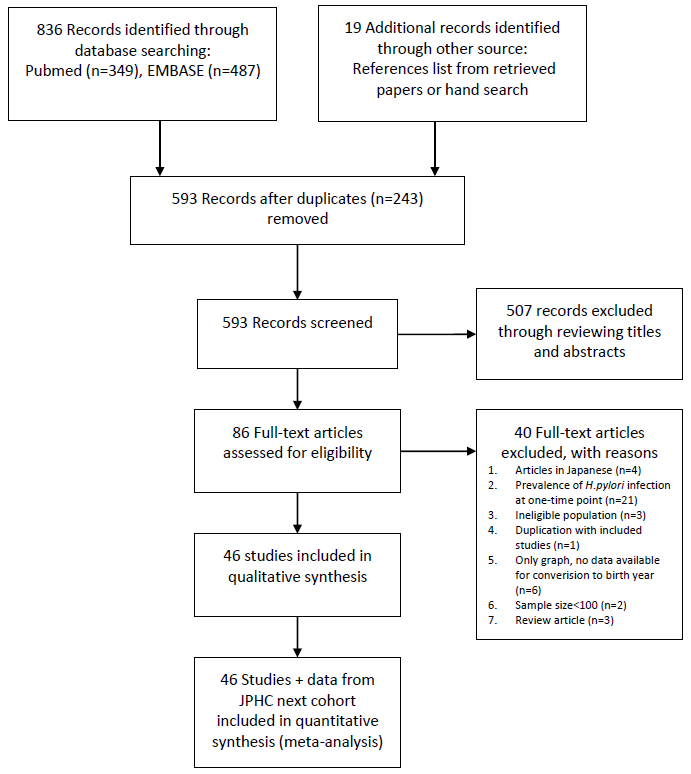
\includegraphics[width=890pt]{images/Figure_1.png}

\caption{Figure 1. PRISMA Flowchart of Study Selection}

\end{block}

\begin{block}{STATISTICAL ANALYSIS (1)}

\begin{itemize}
\item
  More details on how to estimate prevalence of \emph{H. pylori} by
  birth year can be found
  \href{https://winterwang.github.io/For_Inoue_pylori/}{\textbf{here}}\footnote{https://winterwang.github.io/For\_Inoue\_pylori/}.
\item
  Prevalence by birth year was extracted from 47 studies (300 data
  points).
\item
  Observations were weighted by the inverse of the sum of the
  within-study variance and the residual between-study variance using
  the \texttt{meta} package.
\end{itemize}

\end{block}

\column{(\linewidth-1cm)*\real{0.500000}}

\begin{block}{STATISTICAL ANALYSIS (2)}

\begin{itemize}
\item
  Penalized cubic spline was used to model the prevalence as a function
  of birth year in the framework of generalized additive mixed model
  (GAMM) implemented in the \texttt{mgcv} package in R.
\item
  Pre-specified explanatory variables included in the meta-regression
  were as follows:\\
  Study ID, birth year, population source (community-based or
  clinical-based), diagnostic testing (serological test, or others;
  others: urinary assays, salivary assays, stool antigen tests,
  \textsuperscript{13}C-urea breath test, and gastric biopsy), types of
  ELISA kits for measuring \emph{H. pylori} positivity (antigen derived
  from domestic or foreign strains), and data collection period (prior
  to the year 2000, or later than 2000), with \textbf{study ID as a
  random effect} and \textbf{other variables as fixed effects}.
\end{itemize}

\end{block}

\begin{block}{RESULTS}

\begin{itemize}
\item
  Details/characteristics of the studies included in the current
  meta-regression analysis are available
  \href{http://rpubs.com/winterwang/288338}{\textbf{online}}\footnote{http://rpubs.com/winterwang/288338}.
\item
  Summary of the results of risk of bias diagnosis is available
  \href{http://rpubs.com/winterwang/riskofbias}{\textbf{here}}\footnote{http://rpubs.com/winterwang/riskofbias}.
\end{itemize}

\center
\caption{Figure 2: Multivariable adjusted prevalence of \textit{H. pylori} by birth year}
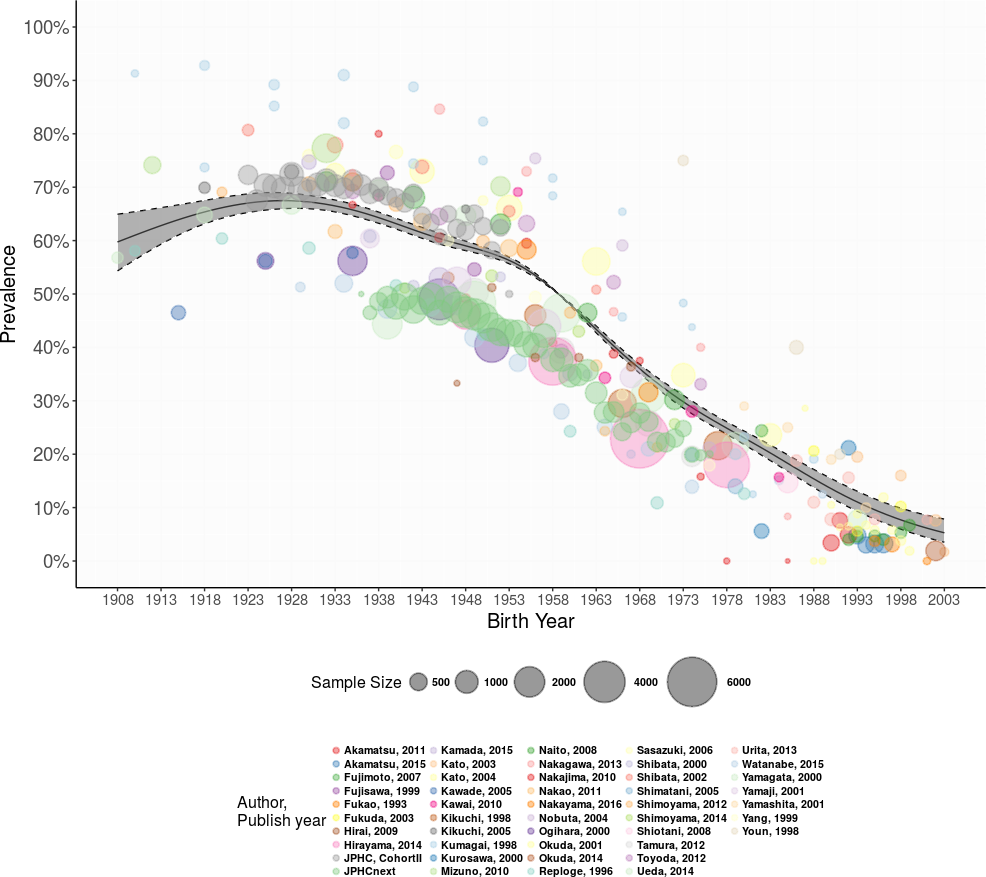
\includegraphics[width=1200pt]{images/Figure2Rev.png}

\begin{table}[]
\captionof{Table 1. Estimated prevalence of \textit{H. pylori} infection by birth year}
\small
\centering
%\caption{My caption}
%\label{my-label}
\begin{tabular}{p{10cm}p{10cm}p{8cm}p{8cm}}
\toprule
\textbf{Birth year} & \textbf{Prevalence} & \textbf{95\% Low} & \textbf{95\% High} \\ \midrule
1908                & 0.597               & 0.543             & 0.649              \\
1909                & 0.603               & 0.553             & 0.651              \\
1910                  & 0.609               & 0.563             & 0.654  \\
...                 & ...              & ...            & ...             \\
1925                & 0.674               & 0.657             & 0.690               \\
1926                & 0.675               & 0.659             & 0.690               \\
\rowcolor[HTML]{FFCB2F} 
1927                & 0.675               & 0.660              & 0.690               \\
1928                & 0.675               & 0.660              & 0.688              \\
...              & ...              & ...            & ...             \\
1950                & 0.582               & 0.574             & 0.590               \\
...              & ...              & ...            & ...             \\
1990                & 0.138               & 0.121             & 0.157              \\
...              & ...              & ...            & ...             \\
1996                & 0.087               & 0.070              & 0.108              \\
1997                & 0.081               & 0.064             & 0.102              \\
\rowcolor[HTML]{FFC702} 
1998                & 0.076               & 0.058             & 0.098              \\
...              & ...              & ...            & ...             \\
2002                & 0.057               & 0.039             & 0.082              \\
2003                & 0.053               & 0.035             & 0.078              \\ \bottomrule
\end{tabular}
\end{table}

\end{block}

\begin{block}{CONCLUSION}

\begin{itemize}
\item
  Prevalence of \emph{H. pylori} infection exhibits \textbf{a birth
  cohort effect} in Japan, with prevalence decreasing steadily in
  individuals born in successive years, \textbf{from 58.2\% in 1950 to
  13.8\% in 1990}.
\item
  Given the fact that the birth-cohort pattern of \emph{H. pylori}
  shapes the trends of gastric cancer over time, our findings help to
  inform screening efforts aimed at prevention and early detection of
  gastric cancer in Japan.
\end{itemize}

\end{block}

\begin{block}{COI Declaration:}

The authors havs no conflict of interest with any corporate
organizations relating to this presentation.

\end{block}

\end{columns}

\end{frame}


\end{document}
